\documentclass[11pt,a4paper]{article}

\usepackage{titling}
\usepackage[hidelinks]{hyperref}
\usepackage{graphicx}
\usepackage{grffile}
\usepackage{float}
\usepackage{geometry}
\usepackage{listings}
\usepackage{parskip}

\setlength{\parindent}{0pt}

\newcommand{\subtitle}[1]{
  \posttitle{
    \par\end{center}
    \begin{center}\large#1\end{center}
    \vskip0.5em}
}

\begin{document}


\title{Hyper Perform\\ Testing Document}
\subtitle{ Organisation: \url{https://github.com/Hyperperform}}
\begin{figure}
			\centering
			
\includegraphics[height=200px]{../Images/CodusMaximus_logo.jpg}
\end{figure}

	
\author{
	\textbf{Developers:} \\
	Rohan Chhipa		\emph{14188377}	\\
	Avinash Singh		\emph{14043778}	\\
	Jason Gordon		\emph{14405025}	\\
	Claudio Da Silva	\emph{14205892}	\\\\
}

\date{\textbf{Updated \today}}

\maketitle
\thispagestyle{empty}
\pagebreak

\tableofcontents
\pagebreak

\section{Introduction}

This document explains implementation of unit tests which were used to test each component in an isolated environment. It also includes an overview of the technologies used as well as instructions on how to execute these tests. \\ 

\section{Purpose}
Hyper Perform is an automated performance tracking tool, which sources information from many different integrations in order to provide information about various employee's performances levels and how they affect the current project's success level. One of the main goals of the system is for the system to be able to be used commercially or in an academic setting. To ensure that each component of the system is decoupled from every other; all aspects of the system are implemented such that they conform to the given contracts. Unit testing is essential to ensure that these contracts are not violated in any way and to ensure that the components that expose the services (REST wrapping) are all working properly before the system is deployed.

\section{Technologies}

Since the system is primarily coded in Java we decided to use the \textit{JUnit testing framework} to carry out the unit tests for each of the components. We also used Spring to allow the use of dependency injection within each test, this allows us to easily inject mocks and test components in an isolated environment. \\

Maven was used as the build tool for this system. When building the system from its source code, all unit tests are automatically executed by Maven.  \\

Another technology which proved useful was a Mock Dispatcher framework which ships with RESTEasy. The mock dispatcher allows one to easily and efficiently test REST API's without having to deploy the component to an application server.

\section{Testing environment}
\begin{itemize}
	\item \textbf{Programming Languages:} Java with JavaEE for the back-end server, front-end relies on AngularJS with Bootstrap, JQuery and Sass.
	
	\item \textbf{Testing frameworks: } Unit testing is done using JUnit. This is combined with Spring, which is used to achieve dependency injection within the unit tests.
	
	\item \textbf{Operating System: } The unit tests are not platform specific. The only requirement in terms of operating systems is that Maven must be supported. If Maven is supported then all unit test dependencies will be downloaded and all the tests will be executed automatically.
	
	\item \textbf{Internet Browsers: } The front-end system supports the latest versions of 
	\textit{Google Chrome} and \textit{Firefox}. There is limited support for other browsers.
\end{itemize}

\section{Execution of unit tests}	
The project has been developed using Maven as a build tool. Thus each unit test can be easily found within the $src/test$ directory of the project. To run the unit tests simply run the following command in terminal (in the same directory as the pom file): \\

$mvn\ clean\ test$ \\\\
All the necessary dependencies for the project will be automatically downloaded.\\ \textbf{Note:} This process of downloading all the project dependencies might consume large amounts of data and time.

\section{Test items}
The following features have been tested in the project:
\begin{itemize}
	\item \textbf{GitListener} - Receives events from GitHub.
	\item \textbf{GitPushEvent} - A POJO that contains information regarding a GitHub push event.
	\item \textbf{TravisListener} - Receives events from Travis CI.
	\item \textbf{AccessListener} - Receives events from Entry/Exit.
	\item \textbf{TravisEvent} - A POJO that contains information regarding a build triggered by a push event from GitHub
	\item \textbf{GitIssueEvent} - A POJO that contains information regarding a GitHub issue that has been created.
	\item \textbf{AccessEvent} - A POJO that contains information regarding access in/out of a building containing a card reader.
	\item \textbf{User} - A POJO that contains information regarding a user who has been registered to the system.
	\item The error codes and exceptions raised when accessing an invalid REST URL.
	 
\end{itemize}

Mock JSON data has been passed to the GitListener, TravisListener and AccessListener classes (into the listen functions). \\\\
Each of these components have dependencies on features such as the messaging queue. All of these features are mocked out to ensure each component is tested in isolation. These features were mocked through dependency injection which was provided by Spring. \\

\section{Features that will not be tested}

Features that have been provided by frameworks will not be tested. Operations such as adding an object to a messaging queue will not be tested. Mapping of JSON data to request objects as this is also done by frameworks.

\section{Components to be mocked}
\begin{itemize}
	\item The JPA entity manager was the first component that was mocked. When testing the possibility for persistence of the POJO's it would be best if the transactions do not affect the database. Thus every transaction that occurs with the mocked entity manager will leave the database system intact and unaffected. An alternate approach could have been to use an in-memory database - such as the one provided by H2 - however this was not deemed necessary. \\
	
	\item The second component to be mocked was the messaging queue provided by ActiveMQ. Once again we do not wish to have unnecessary objects in our queue that might affect actual program execution thus the default queue is replaced with a queue that does not retain objects. \\
	
	\item When testing the event listeners we can't wait for the event emitting systems to send out an event. So we send mock events to the listeners while testing, these mock events are structured in the same manner as their real-world counterparts.
\end{itemize}

\section{Sample tests}
The following figure is the GitListener dependency injected queue which allows multiple events to come through and not be lost and the creation of the entity manager.
\begin{figure}[H]
	\begin{center}
		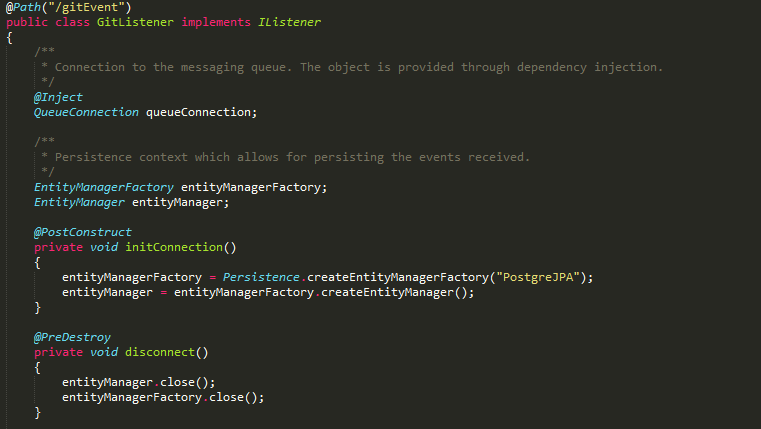
\includegraphics[scale=0.7]{../Images/sample3.PNG}
		\caption{GitListener Dependency injection}
	\end{center}
\end{figure}


The following figure is one of the GitListener Event tests.

\begin{figure}[H]
	\begin{center}
		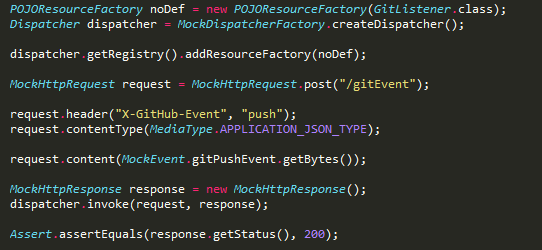
\includegraphics[scale=1.0]{../Images/sample1.PNG}
		\caption{GitListener Push event test}
	\end{center}
\end{figure}
\noindent
In the above figure the $POJOResourceFactory$ and $Dispatcher$ are used to start up an embedded server which will allow for calls to be made to a particular URL, in this case $\backslash$ gitEvent. \\
\\
A post request is created and has the mock event as its content. This post request mirrors the post requests made by GitHub when sending events. Once the mock event data is loaded into the request, the request is sent. At the end, the response objects' HTTP status code is checked. This is checked in an assert statement, the value of the response should be 200 to indicate a successful retrieval. \\

\begin{figure}[H]
	\begin{center}
		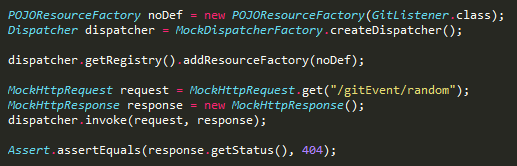
\includegraphics[scale=1.0]{../Images/sample2.PNG}
		\caption{Exception handler for invalid URLs}
	\end{center}
\end{figure}


\section{Unit Test Report}
\subsection{Overview}
All the tests in the system build correctly and pass the test. The only reason that a test may fail is if the database tables have not been created correctly. This may occur due to the fact that these tables are not created using JPA, since JPA destroys and creates the tables upon execution of the command: \textit{mvn clean test}. Travis CI is used on our repository to ensure that the build do pass.

\subsection{Test Cases}

\subsubsection{Test Class 1 - Rest Tests}
%\url{https://github.com/HyperPerform/hyper-perform-server/blob/develop/src/test/java/me/hyperperform/rest/RestTest.java}\\\\
%\textbf{RestTest}
%\begin{itemize}
%	\item $gitIssueEventTest$ - Uses MockEvent.gitIssuesEvent JSON data for issues and tests the Gitlistener.
%	\item $calendarSimpleTest$ - Uses MockEvent.calendarEvents JSON data for Calendar Events and tests the CalendarListener.
%	\item $invalidLinkTest$ - Checks a random invalid rest link to see if it gets a HTTP 404 Error response.
%	\item $travisTest$ - Uses MockEvent.travisEvent JSON data for travis build and tests the Travislistener.
%	\item $timezoneTest$ - Uses MockEvent.alternativeGitPush JSON data for push events with different timezones and tests the Gitlistener for different timezones.
%	\item $gitEventTest$ - Uses MockEvent.gitPushEvent JSON data for push events and tests the Gitlistener.
%\end{itemize}
%Result: \textbf{All Passed}\\\\

\textbf{Test case 1: Git Push Event Test} \\
\textbf{Objective: } This test will ensure that the git listener REST endpoint is working and successfully receives events \\
\textbf{Input: } A mock git push event is send through to the link \\
\textbf{Outcome: } Once the event is sent through, a HTTP 200 response code is expected. \\

\textbf{Test case 2: Git Issues Event Test} \\
\textbf{Objective: } This test will ensure that the git listener REST endpoint is working and successfully accepts git issue events \\
\textbf{Input: } A mock git issue event is send through to the link \\
\textbf{Outcome: } Once the event is sent through, a HTTP 200 response code is expected. \\

\textbf{Test case 3: Invalid link Test} \\
\textbf{Objective: } This test is used to see if an appropriate response is sent for non-existing pages \\
\textbf{Input: } An intentional invalid link is accessed \\
\textbf{Outcome: } An HTTP 404 response code is expected. \\

\textbf{Test case 4: Timezone Test}  \\
\textbf{Objective: } This test checks the  adaptability of the Git Listeners in terms of timezones. Its aims to see if a correct timezone can be parsed from the received data. \\
\textbf{Input: } An alternative git push event is sent through \\
\textbf{Outcome: } An HTTP 200 response code is expected. \\

\textbf{Test case 5: Travis Test}  \\
\textbf{Objective: } This test checks whether or not the travis listener is working. This is tested by sending through a mock event \\
\textbf{Input: } A travis event is sent through \\
\textbf{Outcome: } An HTTP 200 response code is expected. \\

\textbf{Test case 6: Login Test}  \\
\textbf{Objective: } This test checks whether or not the login subsystem under the user management system is working.\\
\textbf{Input: } Mock user details are sent through to the REST endpoint \\
\textbf{Outcome: } An HTTP 200 response code is expected. \\

\textbf{Test case 7: Access Test}  \\
\textbf{Objective: } This test checks whether or not the access listener is working. This is tested by sending through a mock event \\
\textbf{Input: } A mock access event is sent through \\
\textbf{Outcome: } An HTTP 200 response code is expected. 

All these test cases above can be found on the following link: \url{https://github.com/HyperPerform/hyper-perform-server/blob/develop/src/test/java/me/hyperperform/rest/RestTest.java}


\subsubsection{Test Class 2 - User Management Tests}
All mock data can be found in the Appendix.\\
\textbf{Test case 1: Create User Test} \\
\textbf{Objective: } This test will create 2 different users with different roles and persist them into the database. \\
\textbf{Input: } There is no direct input into this test.\\
\textbf{Outcome: } The newly created users are successfully persisted to the database. \\

\textbf{Test case 2: User Test} \\
\textbf{Objective: } Check the integrity of the information of the above users and delete them from the database, to ensure no primary key violation. \\
\textbf{Input: } There is no direct input into this test.\\
\textbf{Outcome: } The newly created users data is as expected and then are successfully deleted from the database. \\


\textbf{Test case 3: Registration Test} \\
\textbf{Objective: } Check to see if a user can be added to the system with all valid information. \\
\textbf{Input: } A mock normalUser event is sent through\\
\textbf{Outcome: } An HTTP 200 response code is expected. There after the test will delete the user to ensure no primary key violation. \\


\textbf{Test case 4: Invalid Name Test} \\
\textbf{Objective: } Check to see if a user can be added to the system with no username. \\
\textbf{Input: }  A mock noUsername event is sent through.\\
\textbf{Outcome: } An HTTP 200 response code is expected with a response message "Error: name" \\

\textbf{Test case 5: Invalid Surname Test} \\
\textbf{Objective: } Check to see if a user can be added to the system with no surname. \\
\textbf{Input: }  A mock noSurname event is sent through.\\
\textbf{Outcome: } An HTTP 200 response code is expected with a response message "Error: surname" \\

\textbf{Test case 6: Invalid Email Test} \\
\textbf{Objective: } Check to see if a user can be added to the system with no email. \\
\textbf{Input: }  A mock noEmail event is sent through.\\
\textbf{Outcome: } An HTTP 200 response code is expected with a response message "Error: email" \\

\textbf{Test case 7: Invalid Role Test} \\
\textbf{Objective: } Check to see if a user can be added to the system with an invalid role. \\
\textbf{Input: }  A mock invalidRole event is sent through.\\
\textbf{Outcome: } An HTTP 200 response code is expected with a response message "Error: Role does not exist" \\


\textbf{Test case 8: Invalid Position Test} \\
\textbf{Objective: } Check to see if a user can be added to the system with an invalid position. \\
\textbf{Input: }  A mock invalidPosition event is sent through.\\
\textbf{Outcome: } An HTTP 200 response code is expected with a response message "Error: Position does not exist" \\


\textbf{Test case 9: Invalid GitUsername Test} \\
\textbf{Objective: } Check to see if a user can be added to the system with no GitUserName. \\
\textbf{Input: }  A mock noGitUsername event is sent through.\\
\textbf{Outcome: } An HTTP 200 response code is expected with a response message "Error: gitUserName" \\


\textbf{Test case 10: Invalid Password} \\
\textbf{Objective: } Check to see if a user can be added to the system with no password. \\
\textbf{Input: }  A mock noPassword event is sent through.\\
\textbf{Outcome: } An HTTP 200 response code is expected with a response message "Error: password" \\

All these test cases above can be found on the following link: \url{https://github.com/HyperPerform/hyper-perform-server/blob/develop/src/test/java/me/hyperperform/user/UserTest.java}

\subsubsection{Test Class 3 - Entry/Exit Tests}	
\textbf{Test case 1: Create Access Event Test} \\
\textbf{Objective: } The purpose of this test is to be a precursor to see if an access event can be created and then persisted to the database. \\
\textbf{Input: } There is no direct input to the test. \\
\textbf{Outcome: } The following are expected outcomes for the functionality: 
\begin{enumerate}
	\item The access event should be persisted in the database. This is tested in test case 3\\
	%		\item The test should assert that the email address and timestamp is the same as the ones persisted.\\
\end{enumerate}
\noindent
\textbf{Test case 2: POJO Test} \\
\textbf{Objective: } The purpose of this test is to check if the access event from test case 1 mapped correctly to the \textit{AccessEvent} POJO. \\
\textbf{Input: } There is no direct input to the test. \\
\textbf{Outcome: } The following are expected outcomes for the functionality:
\begin{enumerate}
	\item Should assert that the expected name is the same as the name mapped on to the POJO.
	\item Should assert that the expected email address is the same as the email address mapped on to the POJO.
	\item Should assert that the expected surname is equal to the surname mapped on to the POJO.
	\item Should assert that the expected userID is equal to the userID mapped on to the POJO.
	\item Should assert that the expected deviceID is equal to the deviceID mapped on to the POJO.
	\item Should assert that the expected day is equal to the day mapped on to the POJO.
	\item Should assert that the expected timestamp is equal to the timestamp mapped on to the POJO.\\
\end{enumerate}

\noindent
\textbf{Test case 3: Querying the database test} \\
\textbf{Objective: } The purpose of this test is to query the AccessEvent table in the database and check if the access event from test case 1 persisted correctly to the database. \\
\textbf{Input: } There is no direct input to the test. \\
\textbf{Outcome: } The following are expected outcomes for the functionality:
\begin{enumerate}
	\item Should assert that the expected name is equal to that of the one persisted.
	\item Should assert that the expected email address is equal to that of the one persisted.
	\item Should assert that the expected surname is equal to that of the one persisted.
	\item Should assert that the expected userID is equal to that of the one persisted.
	\item Should assert that the expected deviceID is equal to that of the one persisted.
	\item Should assert that the expected day is equal to that of the one persisted.
	\item Should assert that the expected timestamp is equal to that of the one persisted.\\
\end{enumerate}

All these test cases can be found on the following link:
\url{https://github.com/HyperPerform/hyper-perform-server/blob/develop/src/test/java/me/hyperperform/event/EntryExitTest.java}

\subsubsection{Test Class 4 - Persistence Tests}	
\textbf{Test case 1: Create Travis Event Test} \\
\textbf{Objective: } The purpose of this test is to see if a Travis Event can be created, mapped to the POJO and then persisted to the database. \\
\textbf{Input: } There is no direct input to the test. \\
\textbf{Outcome: } The following are expected outcomes for the functionality: 
\begin{enumerate}
	\item The created Travis event should be persisted to the database. This is tested in test case 9.\\
\end{enumerate}
\noindent
\textbf{Test case 2: Create Git Issue Test} \\
\textbf{Objective: } The purpose of this test is to see if a Git Issue Event can be created, mapped to the POJO and then persisted to the database. \\
\textbf{Input: } There is no direct input to the test. \\
\textbf{Outcome: } The following are expected outcomes for the functionality: 
\begin{enumerate}
	\item The Git Issue that was created should be persisted to the database. This is queried and tested in test case 8.\\
\end{enumerate}
\noindent
\textbf{Test case 3: Create Git Push Test} \\
\textbf{Objective: } The purpose of this test is to see if a Git Push Event can be created, mapped to the POJO and then persisted to the database. \\
\textbf{Input: } There is no direct input to the test. \\
\textbf{Outcome: } The following are expected outcomes for the functionality: 
\begin{enumerate}
	\item The Git Push (along with their commits) that was created should be persisted to the database. This is queried and tested in test case 7.\\
\end{enumerate}
\noindent
\textbf{Test case 4: Travis Event POJO Test} \\
\textbf{Objective: } The purpose of this test is to see if the Travis Event in test case 1 mapped correctly to the POJO. \\
\textbf{Input: } There is no direct input to the test. \\
\textbf{Outcome: } The following are expected outcomes for the functionality:
\begin{enumerate}
	\item Should assert that the expected committer is equal to that of the one mapped onto the POJO.
	\item Should assert that the expected branch is equal to that of the one mapped onto the POJO.
	\item Should assert that the expected status of the issue is equal to that of the one mapped onto the POJO.
	\item Should assert that the expected timestamp is equal to that of the one mapped onto the POJO.
	\item Should assert that the expected repository name is equal to that of the one mapped onto the POJO.\\
\end{enumerate}
\noindent
\textbf{Test case 5: Git Issue POJO Test} \\
\textbf{Objective: } The purpose of this test is to see if the Git Issue in test case 2 mapped correctly to the POJO. \\
\textbf{Input: } There is no direct input to the test. \\
\textbf{Outcome: } The following are expected outcomes for the functionality:
\begin{enumerate}
	\item Should assert that the expected issueId is equal to that of the one mapped onto the POJO.
	\item Should assert that the expected action is equal to that of the one mapped onto the POJO.
	\item Should assert that the expected repository name is equal to that of the one mapped onto the POJO.
	\item Should assert that the timestamp that was mapped onto the POJO is not null.
	\item Should assert that the expected timestamp is equal to that of the one mapped onto the POJO.
	\item Should assert that the expected assignee of the issue is equal to that of the one mapped onto the POJO.
	\item Should assert that the expected creator of the issue is equal to that of the one mapped onto the POJO.\\
\end{enumerate}
\noindent
\textbf{Test case 6: Git Push POJO Test} \\
\textbf{Objective: } The purpose of this test is to see if the Git Push Event in test case 3 mapped correctly to the POJO. \\
\textbf{Input: } There is no direct input to the test. \\
\textbf{Outcome: } The following are expected outcomes for the functionality:
\begin{enumerate}
	\item Should assert that the expected repository name/path is equal to that of the one mapped onto the POJO.
	\item Should assert that the expected timestamp is equal to that of the one mapped onto the POJO.
	\item Should assert that the expected username is equal to that of the one mapped onto the POJO.
	\item Should assert that the commit size that was mapped onto the POJO cannot be equal to zero.
	\item Should assert that the expected commit size is equal to that of the one mapped onto the POJO.\\
\end{enumerate}
\noindent
\textbf{Test case 7: Git Push Query Test} \\
\textbf{Objective: } The purpose of this test is to query the GitPush table in the database and check if the GitPush event from test case 3 persisted correctly to the database. \\
\textbf{Input: } There is no direct input to the test. \\
\textbf{Outcome: } The following are expected outcomes for the functionality:
\begin{enumerate}
	\item Should assert that the query from the database does return results thus the number of results is not equal to 0 (zero).
	\item Should assert that the expected repository name/path is equal to that of the one persisted.
	\item Should assert that the expected Date (extracted from the timestamp) is equal to that of the one persisted.
	\item Should assert that the expected username is equal to that of the one persisted.
	\item Should assert that the commit size that was persisted to the database cannot be equal to zero.
	\item Should assert that the expected commit size is equal to that of the one persisted.\\
\end{enumerate}
\noindent
\textbf{Test case 8: Git Issue Query Test} \\
\textbf{Objective: } The purpose of this test is to query the GitIssue table in the database and check if the GitIssue event from test case 2 persisted correctly to the database. \\
\textbf{Input: } There is no direct input to the test. \\
\textbf{Outcome: } The following are expected outcomes for the functionality:
\begin{enumerate}
	\item Should assert that the query from the database does return results (i.e. the number of results is not equal to 0 (zero)).
	\item Should assert that the expected action is equal to that of the one persisted.
	\item Should assert that the expected repository name is equal to that of the one persisted.
	\item Should assert that the expected timestamp is equal to that of the one persisted.
	\item Should assert that the expected assignee of the issue is equal to that of the one persisted.
	\item Should assert that the expected creator of the issue is equal to that of the one persisted.\\
\end{enumerate}
\noindent
\textbf{Test case 9: Travis Event Query Test} \\
\textbf{Objective: } The purpose of this test is to query the TravisEvent table in the database and check if the Travis event from test case 1 persisted correctly to the database. \\
\textbf{Input: } There is no direct input to the test. \\
\textbf{Outcome: } The following are expected outcomes for the functionality:
\begin{enumerate}
	\item Should assert that the query from the database does return results thus the number of results is not equal to 0 (zero).
	\item Should assert that the expected committer is equal to that of the one persisted.
	\item Should assert that the expected branch, on which the builds was done, is equal to that of the one persisted.
	\item Should assert that the expected status of the build is equal to that of the one persisted.
	\item Should assert that the expected timestamp is equal to that of the one persisted.
	\item Should assert that the expected repository name is equal to that of the one persisted.\\
\end{enumerate}
All these test cases can be found on the following link:
\url{https://github.com/HyperPerform/hyper-perform-server/blob/develop/src/test/java/me/hyperperform/event/PersistenceTest.java}\\

\begin{figure}[H]
	\centering
	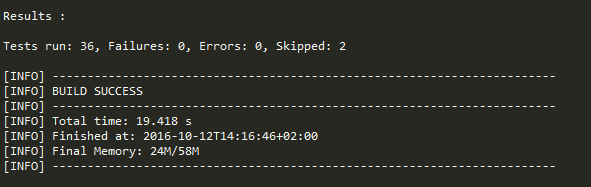
\includegraphics[scale=1.0]{../Images/Build_Status}
	\caption{Final Build Status}
\end{figure}

\section{Conclusion}
All 36 tests that have been run have passed (as shown by Figure 4 above). Additionally this was confirmed by Travis CI which we have used on our repository to make sure that there are no compilation failures or test failures. The limitations to these tests are the fact that they require the relevant tables to already exist in the Postgres database because otherwise JPA will not create these tables and will try use tables that do not already exist, resulting in an error. A work around for this is to write a script or a unit test that will create these tables if they don't exist before the rest of the unit tests are executed.

\newpage

\section{Appendix}

\subsection{Mock Events}
\textbf{Please note that some of these mock events are very large. Due to this redundant data has been removed from the events so that they can be presented in this document.} \\

The fully detailed mock events can be found through the following link: \url{https://github.com/HyperPerform/hyper-perform-server/blob/develop/src/test/java/me/hyperperform/event/MockEvent.java} \\

\begin{figure}[H]
	\centering
	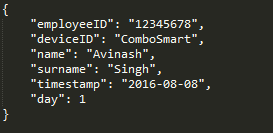
\includegraphics[scale=1.0]{../Images/accessEvent}
	\caption{Access event payload}
\end{figure}
 
\begin{figure}[H]
	\centering
	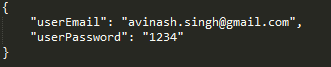
\includegraphics[scale=1.0]{../Images/loginEvent}
	\caption{Login payload}
\end{figure}

\begin{figure}[H]
	\centering
	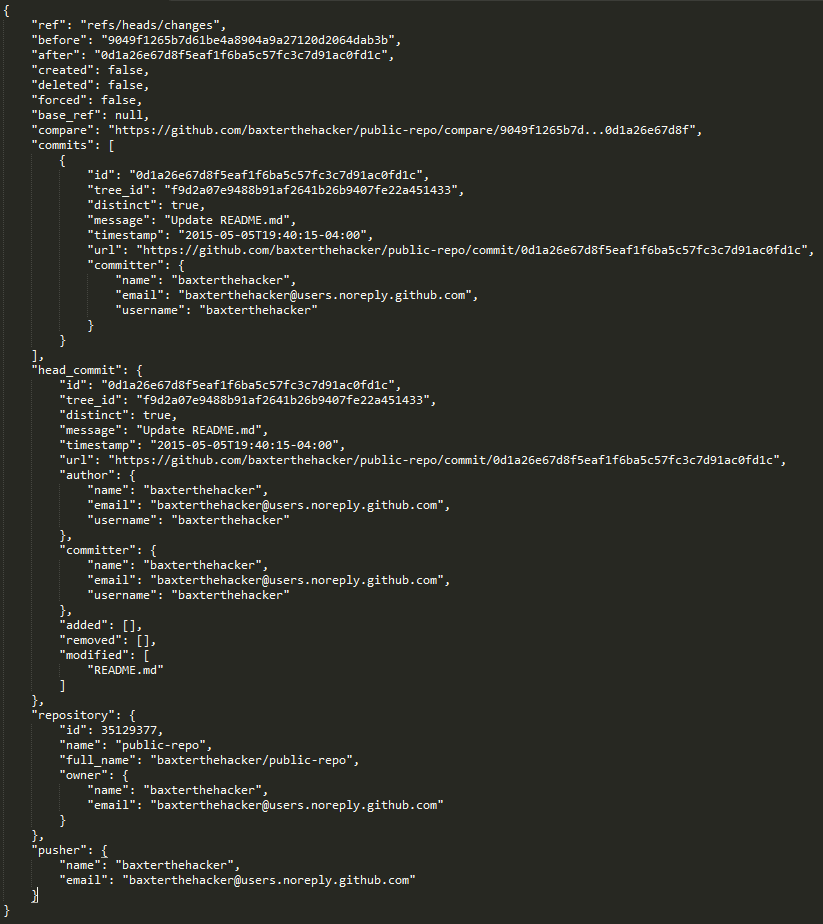
\includegraphics[width=\linewidth]{../Images/gitpush}
	\caption{Git push event payload}
\end{figure}

\begin{figure}[H]
	\centering
	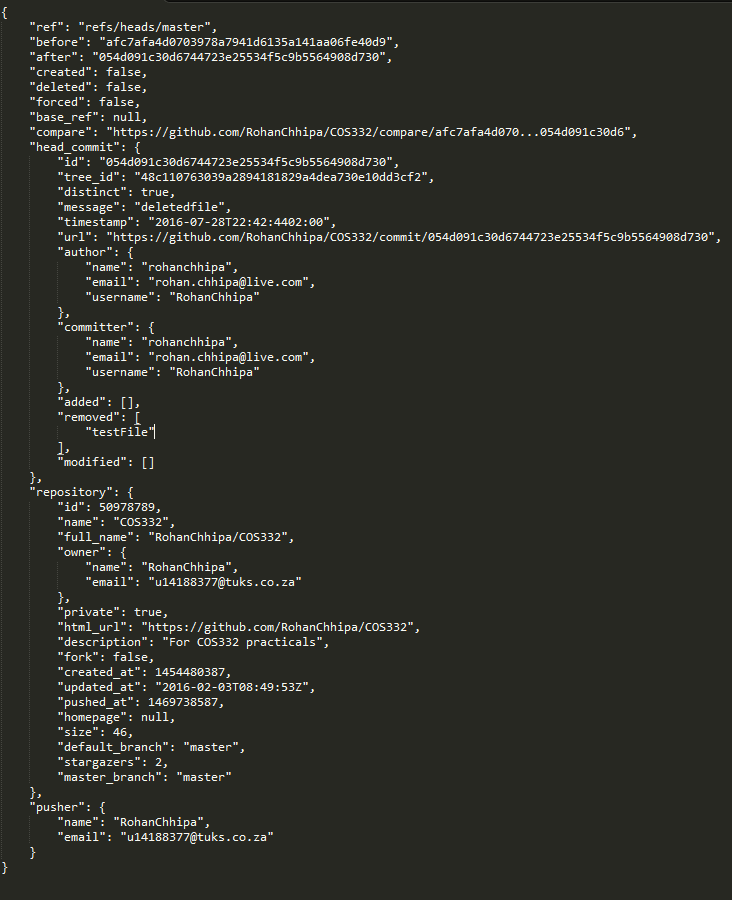
\includegraphics[width=\linewidth]{../Images/altgitpush}
	\caption{Alternative Git push event payload}
\end{figure}

\begin{figure}[H]
	\centering
	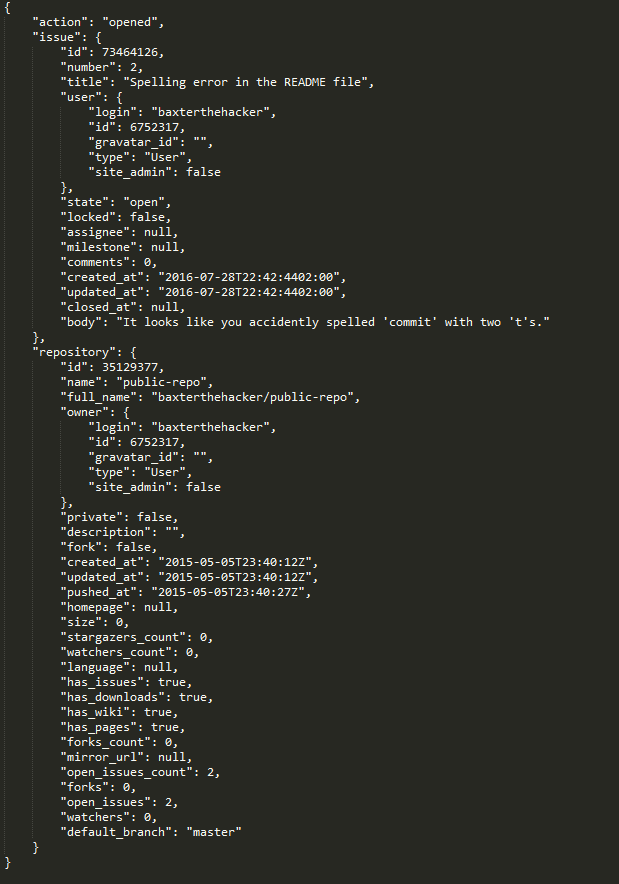
\includegraphics[width=\linewidth]{../Images/gitissues}
	\caption{Git issues event payload}
\end{figure}

\begin{figure}[H]
	\centering
	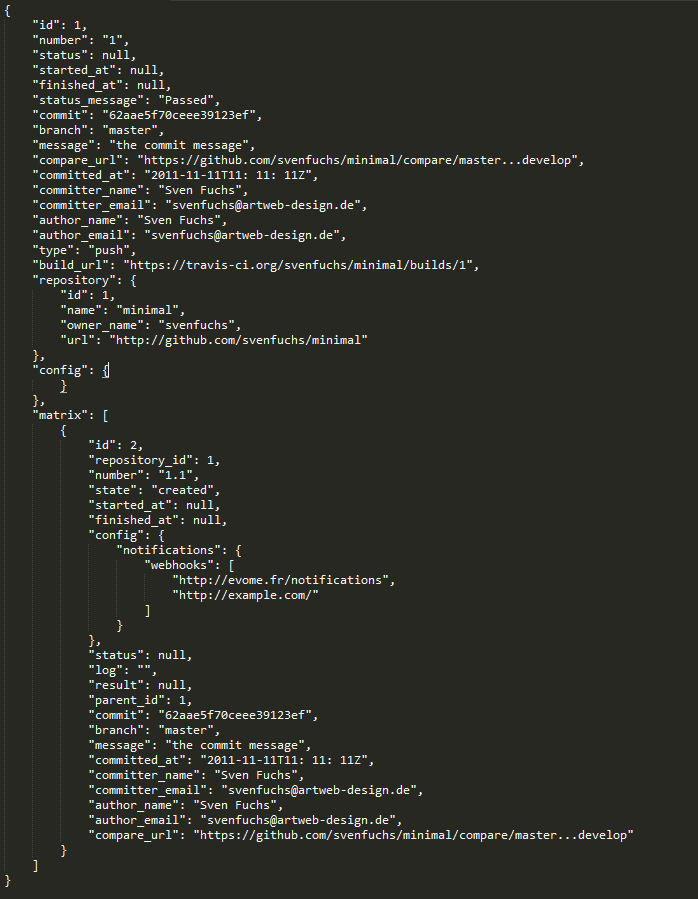
\includegraphics[width=\linewidth]{../Images/travisEvent}
	\caption{Travis build event payload}
\end{figure}

\begin{figure}[H]
	\centering
	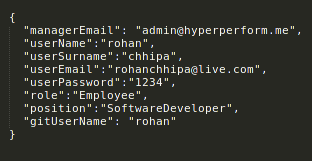
\includegraphics[width=.5\linewidth]{../Images/normaluser}
	\caption{Normal User}
\end{figure}

\begin{figure}[H]
	\centering
	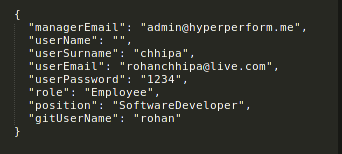
\includegraphics[width=.5\linewidth]{../Images/nousername}
	\caption{No Username}
\end{figure}


\begin{figure}[H]
	\centering
	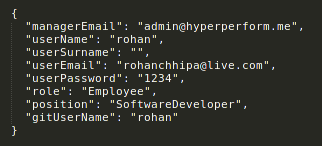
\includegraphics[width=.5\linewidth]{../Images/nosurname}
	\caption{No Surname}
\end{figure}

\begin{figure}[H]
	\centering
	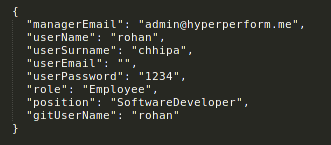
\includegraphics[width=.5\linewidth]{../Images/noemail}
	\caption{No Email}
\end{figure}

\begin{figure}[H]
	\centering
	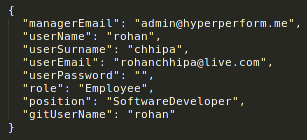
\includegraphics[width=.5\linewidth]{../Images/noPass}
	\caption{No Password}
\end{figure}


\begin{figure}[H]
	\centering
	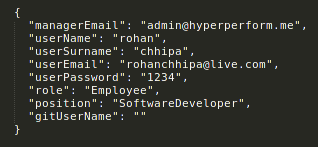
\includegraphics[width=.5\linewidth]{../Images/nogit}
	\caption{No GitUsername}
\end{figure}

\begin{figure}[H]
	\centering
	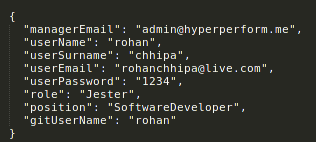
\includegraphics[width=.5\linewidth]{../Images/role}
	\caption{Invalid Role}
\end{figure}

\begin{figure}[H]
	\centering
	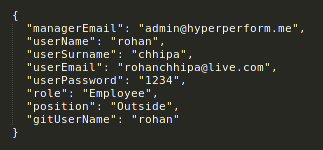
\includegraphics[width=.5\linewidth]{../Images/position}
	\caption{Invalid Position}
\end{figure}

\end{document}
